\documentclass[11pt,a4paper]{article}

\usepackage[margin=1in]{geometry}
\usepackage{amsmath}
\usepackage{amssymb}
\usepackage{graphicx}
\usepackage{booktabs}
\usepackage{xcolor}
\usepackage{enumitem}
\usepackage{subcaption}
\usepackage{float}
\usepackage{titlesec}
\usepackage[hidelinks]{hyperref}

\titleformat{\section}{\large\bfseries\color{blue!45!black}}{\thesection}{0.6em}{}
\titleformat{\subsection}{\normalsize\bfseries\color{blue!35!black}}{\thesubsection}{0.6em}{}

\title{

\includegraphics[height=2cm]{logos/ufrn.png}\hspace{1.5cm}  
\includegraphics[height=2cm]{logos/dimap.png}\\[1em]
  {\normalsize UNIVERSIDADE FEDERAL DO RIO GRANDE DO NORTE\\
  Centro de Ciências Exatas e da Terra - Departamento de Informática e Matemática Aplicada\\
  DIM0411 - Image Processing - Prof. Bruno Motta de Carvalho}\\[1em]
  \Large\textbf{Image Compression Using the Discrete Cosine Transform (DCT)}\\[0.3em]
  \large\itshape Transform-Based (Lossy) Image Compression Project
}
\author{Eduardo Marinho & Kael Paraguassu}
\date{July 09, 2026}

\begin{document}

\maketitle

\section{Introduction}

This project implements a lossy, transform-based image compression pipeline based on the same block-wise Discrete Cosine Transform (DCT) scheme used by the JPEG standard. A grayscale image is divided into $8\times8$ pixel blocks, each block is transformed into the frequency domain, its coefficients are quantized (which discards information and introduces sparsity), and the image is then reconstructed through inverse quantization and inverse DCT. The trade-off between reconstruction quality and compression is controlled by a user-defined compression factor that scales a standard JPEG luminance quantization matrix.

The program was implemented in C++ using OpenCV strictly for the image I/O and matrix display, all DCT, quantization, and metric computations were implemented from scratch. Quality is evaluated with the Mean Squared Error (MSE) and Peak Signal-to-Noise Ratio (PSNR), and the compression rate (CR) is estimated from the number of coefficients that survive quantization.

\section{Methodology}

\subsection{Pipeline Overview}

The image is read in grayscale and zero-padded so that both dimensions become multiples of 8. The padded image is then processed independently, block by block ($8\times8$ pixels), through the following stages:

\begin{itemize}[topsep=2pt,itemsep=2pt]
  \item \textbf{Forward DCT} $\xrightarrow{}$ convert the pixel block to the frequency domain.
  \item \textbf{Quantization} $\xrightarrow{}$ divide each frequency coefficient by a (scaled) quantization step and round to the nearest integer, discarding small/high-frequency components.
  \item \textbf{Inverse quantization} $\xrightarrow{}$ multiply the quantized coefficients back by the same quantization step.
  \item \textbf{Inverse DCT} $\xrightarrow{}$ convert the dequantized coefficients back to the spatial (pixel) domain.
\end{itemize}

Reconstructed blocks are reassembled into the final image, and the original padding is cropped away before saving the output and computing quality metrics.

\subsection{Discrete Cosine Transform}

Before transforming, each pixel value is level-shifted by subtracting 128 so that values are centered around zero. The 2D forward DCT of an $8\times8$ block $f(x,y)$ is computed as:

\begin{equation}
F(u,v) = \frac{1}{4}\, C(u)\, C(v) \sum_{x=0}^{7}\sum_{y=0}^{7} \big[f(x,y) - 128\big] \cos\!\left[\frac{(2x+1)u\pi}{16}\right]\cos\!\left[\frac{(2y+1)v\pi}{16}\right]
\end{equation}

where $x,y,u,v \in \{0,\dots,7\}$, and
\begin{equation}
C(k) =
\begin{cases}
1/\sqrt{2}, & k = 0 \\
1, & k \neq 0
\end{cases}
\end{equation}

The inverse DCT applies the same cosine basis in reverse, adds 128 back to undo the level shift, and clips the result to the valid $[0,255]$ range before rounding to an integer pixel value.

\subsection{Quantization}

Quantization uses the standard JPEG luminance quantization matrix $Q$ ($8\times8$), scaled by the user defined compression factor $f$: each step is
\begin{equation}
Q'(i,j) = \max\big(1,\ Q(i,j)\cdot f\big).
\end{equation}
Each DCT coefficient is divided by its corresponding step and rounded:
\begin{equation}
F_q(u,v) = \operatorname{round}\!\left[\frac{F(u,v)}{Q'(i,j)}\right].
\end{equation}
Larger values of $f$ enlarge the quantization steps, driving more coefficients, especially the high-frequency ones, to zero. This is what produces compression, the fraction of nonzero coefficients that remain after this step directly determines the achievable compression rate. Smaller values of $f$ preserve more coefficients and produce reconstructed images that more closely resemble the original.

\subsection{Reconstruction}

To reconstruct an approximation of the original block, each quantized coefficient is multiplied back by the same step used to quantize it (dequantization: $\hat F(u,v) = F_q(u,v)\cdot Q'(i,j)$), and the inverse DCT described in Section~2.2 is applied to recover the pixel block.

\subsection{Evaluation Metrics}

Reconstruction error is measured with the Mean Squared Error between the original image $I$ and the reconstructed image $K$ (both $m \times n$):

\begin{equation}
\text{MSE} = \frac{1}{m \cdot n} \sum_{i=0}^{m-1}\sum_{j=0}^{n-1} \big[I(i,j) - K(i,j)\big]^2
\end{equation}

Quality is then reported as the Peak Signal-to-Noise Ratio, in decibels, using $\text{Max}_I = 255$ for an 8-bit image:

\begin{equation}
\text{PSNR} = 20 \cdot \log_{10}\!\left(\frac{\text{Max}_I}{\sqrt{\text{MSE}}}\right)
\end{equation}

The compression rate is estimated as the ratio between the uncompressed size (total number of pixels) and the number of nonzero quantized coefficients retained across all blocks. This isolates and measures the sparsification effect of quantization, it does not include the additional gain that a final entropy-coding stage (e.g.\ Huffman or run-length coding, as in real JPEG) would provide on top of it.

\section{Results}

The program was used to compress a sample grayscale test image using four compression factors, ranging from a light setting (1.0) to a heavy setting (8.0), to illustrate the quality/compression trade-off described in Section~2.3.

\subsection{Input Image}

\begin{figure}[h]
    \centering
    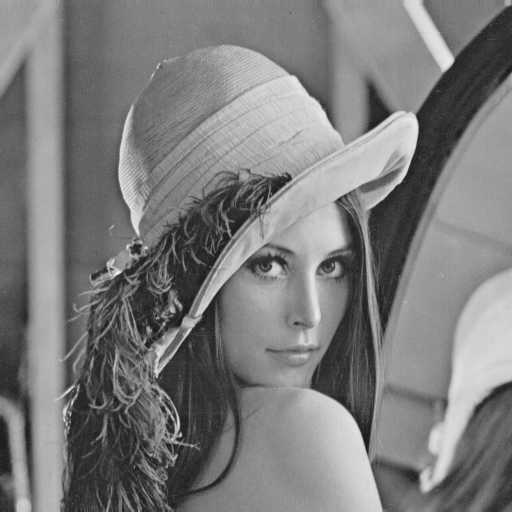
\includegraphics[width=0.8\linewidth]{../data/input/Lenna_gray.jpg}
    \caption{Original grayscale input image.}
    \label{fig:placeholder}
\end{figure}

\subsection{Output Images at Different Compression Levels}
\begin{figure}[H]
    \centering

    \begin{subfigure}{0.48\textwidth}
        \centering
        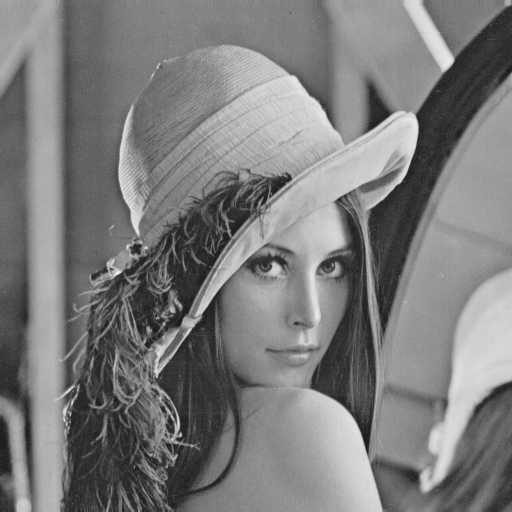
\includegraphics[width=\linewidth]{../data/output/Lena_compressed1.jpg}
        \caption{Compression factor $=$ 1}
    \end{subfigure}
    \hfill
    \begin{subfigure}{0.48\textwidth}
        \centering
        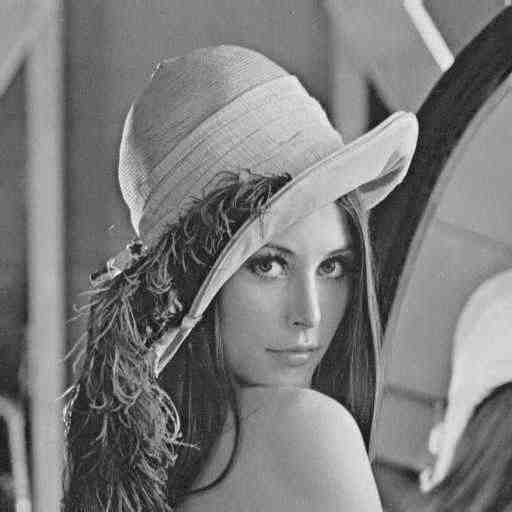
\includegraphics[width=\linewidth]{../data/output/Lena_compressed2.jpg}
        \caption{Compression factor $=$ 2}
    \end{subfigure}
    \begin{subfigure}{0.48\textwidth}
        \centering
        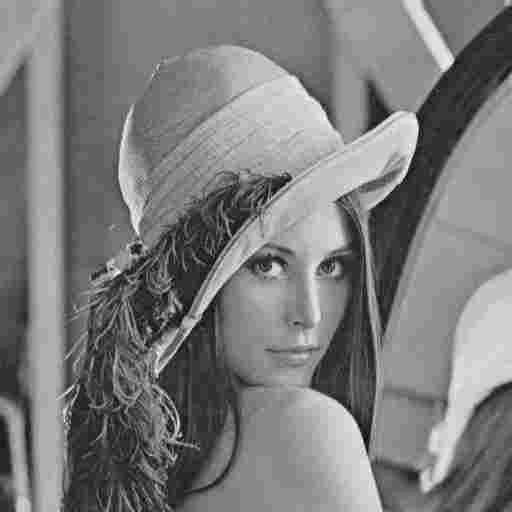
\includegraphics[width=\linewidth]{../data/output/Lena_compressed4.jpg}
        \caption{Compression factor $=$ 4}
    \end{subfigure}
    \hfill
    \begin{subfigure}{0.48\textwidth}
        \centering
        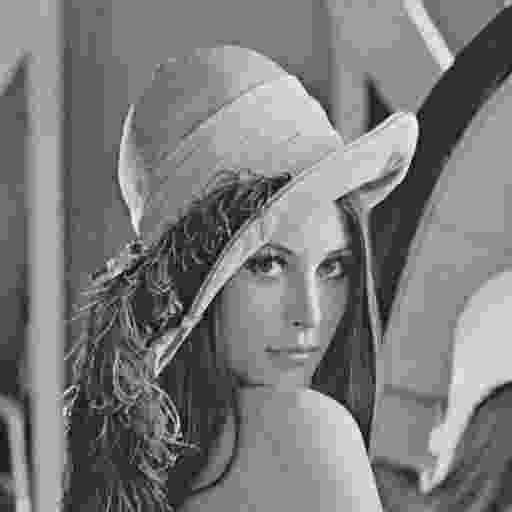
\includegraphics[width=\linewidth]{../data/output/Lena_compressed8.jpg}
        \caption{Compression factor $=$ 8}
    \end{subfigure}

    \caption{Reconstructed image at compression factors 1.0, 2.0, 4.0, and 8.0, respectively.}
    \label{fig:lena-comparison}
\end{figure}

\subsection{Quantitative Results}

\begin{center}
\renewcommand{\arraystretch}{1.3}
\begin{tabular}{lccc}
\toprule
\textbf{Compression Factor} & \textbf{MSE} & \textbf{PSNR (dB)} & \textbf{Compression Ratio} \\
\midrule
1.0        & 0.00965 & 68.285 & 9.14732x \\
2.0        & 24.7137 & 34.2014 & 12.2669x \\
4.0        & 44.9737 & 31.6012 & 21.9221x \\
8.0        & 88.5617 & 28.6583 & 35.3627x \\
\bottomrule
\end{tabular}
\end{center}

The results confirm the expected quality/compression trade-off, however, they reveal to have a non-linear compression rate and data loss. At factor 1.0, reconstruction results highly resemble the original image, since the quantization steps are close to the base JPEG matrix and almost every DCT coefficient survives. Intuitively, this is also the setting with the lowest compression ratio ($9.15\times$). Raising the factor to 2.0 causes a disproportionate drop in quality, as PSNR drops by over 34~dB ($68.285 \rightarrow 34.201$~dB), for a comparatively small gain in compression ratio ($9.15\times \rightarrow 12.27\times$). Beyond that point the trade-off becomes more favorable: going from factor 2.0 to 8.0 nearly triples the compression ratio ($12.27\times \rightarrow 35.36\times$) while PSNR falls by only about 5.5~dB ($34.201 \rightarrow 28.658$~dB), with MSE increasing more gradually ($24.71 \rightarrow 88.56$) than in the initial jump.
 
This pattern indicates that most of the perceptible quality loss occurs when moving from low to moderate compression, as many mid- and high-frequency coefficients are first rounded to zero. After that, increasing the compression factor mainly removes coefficients with less significant information, resulting in smaller PSNR reductions. Visually, this is consistent with sharp detail and edges being preserved at factor 1.0, while $8\times8$ blocking artifacts and loss of fine texture become increasingly visible from factor 2.0 onward, most noticeably at factor 8.0. 

The quantitative results clearly corroborate with our visual observations, since the image 'a' (compression rate = 1) is almost equal to the original image, and, as the compression factor increases, the image quality decays significantly.

\section{Conclusion}
The experiments confirm the fundamental trade-off inherent to DCT-based lossy compression: increasing the compression factor increases the achievable compression ratio at the cost of reconstruction fidelity, but the two do not scale together at a constant rate. The quantitative results suggests that, for this image, a factor around 2.0 already achieves most of the compression gain before the improvements in compression rate become less significant. Because of that, pushing further to factor 8.0 is only worthwhile when a much higher compression ratio is required and the accompanying blocking artifacts and loss of fine detail are acceptable.

\end{document}
